% VUT FIT MITAI
% MSZ 2021/2022
% Author: Vladimir Dusek
% Login: xdusek27

%%%%%%%%%%%%%%%%%%%%%%%%%%%%%%%%%%%%%%%%%%%%%%%%%%%%%%%%%%%%%%%%%%%%%%%%%%%%%%%%

% Path to figures
\graphicspath{{tin/zasobnikove_automaty/figures}}

%%%%%%%%%%%%%%%%%%%%%%%%%%%%%%%%%%%%%%%%%%%%%%%%%%%%%%%%%%%%%%%%%%%%%%%%%%%%%%%%

\chapter{TIN~--~Zásobníkové automaty (jazyky přijímané ZA, varianty ZA).}

%%%%%%%%%%%%%%%%%%%%%%%%%%%%%%%%%%%%%%%%%%%%%%%%%%%%%%%%%%%%%%%%%%%%%%%%%%%%%%%%

\section{Zdroje}

\begin{compactitem}
    \item \path{tin_2021_merged.pdf}
    \item \path{TIN_2020-10-06.mp4}
    \item \path{TIN_2020-10-13.mp4}
\end{compactitem}

%%%%%%%%%%%%%%%%%%%%%%%%%%%%%%%%%%%%%%%%%%%%%%%%%%%%%%%%%%%%%%%%%%%%%%%%%%%%%%%%

\section{Zásobníkový automat}

Zásobníkové automaty dokáží přijímat bezkontextové jazyky.

\paragraph{Definice} Zásobníkový automat (ZA) je sedmice $M = (Q, \Sigma, \Gamma, \delta, q_0, Z_0, F)$, kde \begin{compactitem}
    \item $Q$ je konečná množina stavů;
    \item $\Sigma$ je vstupní abeceda;
    \item $\Gamma$ je zásobníková abeceda;
    \item $\delta$ je přechodová funkce (parciální funkce), \begin{compactitem}
        \item $\delta : Q \times ( \Sigma \cup \{ \epsilon \} ) \times \Gamma \rightarrow 2^{Q \times \Gamma^*}$;
    \end{compactitem}
    \item $q_0$ je výchozí stav, \begin{compactitem}
        \item $q_0 \in Q$;
    \end{compactitem}
    \item $Z_0$ je výchozí symbol na zásobníku, \begin{compactitem}
        \item $Z_0 \in \Gamma$;
    \end{compactitem}
    \item $F$ je množina koncových stavů, \begin{compactitem}
        \item $F \subseteq Q$;
    \end{compactitem}
\end{compactitem}

\paragraph{Konfigurace} Konfigurace ZA je trojice $(q, w, \alpha) \in Q \times \Sigma^* \times \Gamma^*$, kde \begin{compactitem}
    \item $q$ je aktuální stav;
    \item $w$ je nezpracovaná část vstupního řetězce;
    \item $\alpha$ je obsah zásobníku.
\end{compactitem}

\paragraph{Počáteční konfigurace} Počáteční konfigurace ZA je taková konfigurace $(q, w, \alpha)$, kde $w \in \Sigma^*$ je vstupní řetězec, $q \in Q$ je výchozí stav a $\alpha = Z \in \Gamma$ je výchozí symbol na zásobníku.

\paragraph{Koncová konfigurace} Koncová konfigurace ZA je taková konfigurace $(q, w, \alpha)$, kde $q \in F$, $w = \epsilon$ a $\alpha \in \Gamma^*$.

\paragraph{Přechod} Přechod (krok výpočtu) ZA je binární relace (značíme $\vdash$) na množině konfigurací $\vdash ~ \subseteq (Q \times \Sigma^* \times \Gamma^*)^2$, taková, že $$ (q, w, \alpha) \vdash (q', w', \alpha') \Leftrightarrow \exists a \in (\Sigma \cup \epsilon), ~ \exists Z \in \Gamma, ~ \exists \beta, \gamma \in \Gamma^* ~:~ $$

$$ ~:~ w = aw' \land \alpha = Z \beta \land \alpha' = \gamma \beta \land (q', \gamma) \in \delta(q, a, Z) $$

\begin{figure}[H]
    \centering
    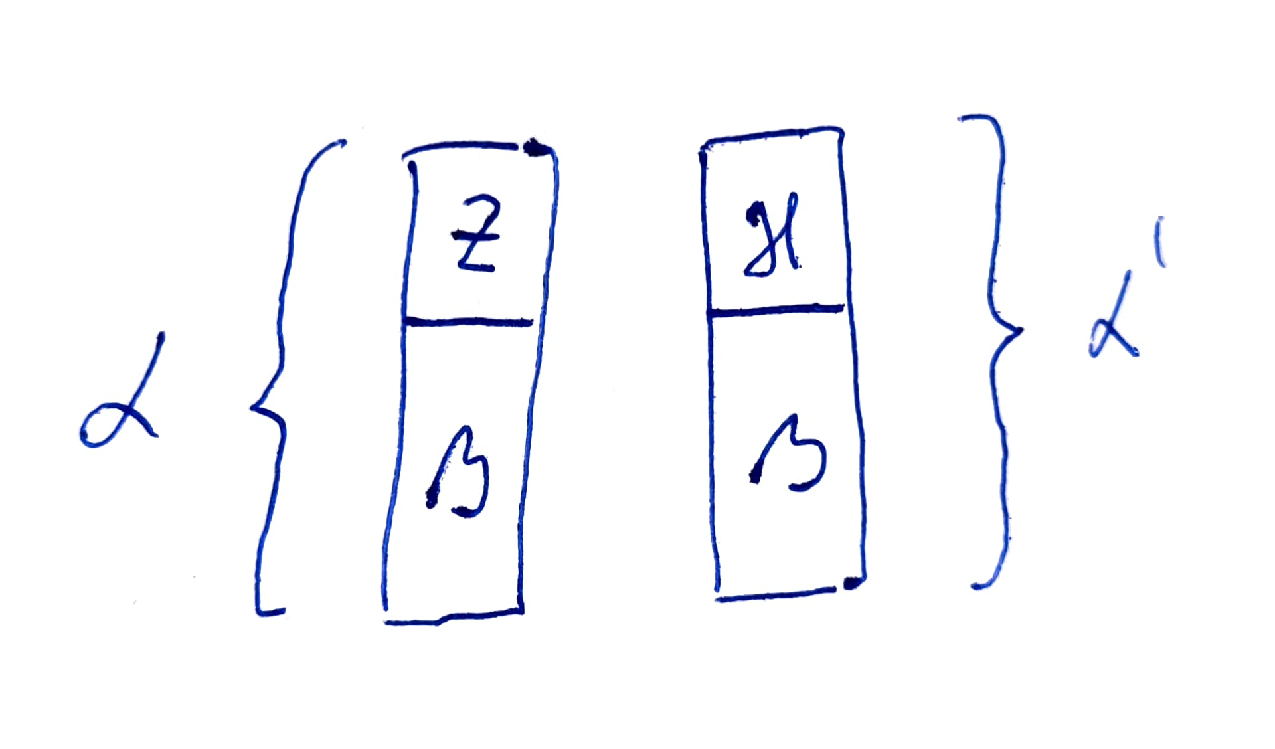
\includegraphics[width=0.35\linewidth]{za_prechod_zasobnik.pdf}
    \caption{Stav zásobníku během přechodu ZA. Platí $Z \in \Gamma,~ \alpha, \alpha', \beta, \gamma \in \Gamma^*$.}
\end{figure}

\paragraph{Jazyk přijímaný} Mějme ZA $M = (Q, \Sigma, \Gamma, \delta, q_0, Z_0, F)$ a jazyk $L(M)$, který je přijímaný ZA $M$. $$ L(M) = \{ w ~|~ w \in \Sigma^* \land (q_0, w, Z_0) \vdash^* (q_f, \epsilon, \epsilon) \land q_f \in F \}$$ Avšak existují různé varianty. ZA může přijímat i v $q_f \in F$: pouze při vyprázdnění vstupu, nebo pouze při vyprázdnění zásobníku a nebo při vyprázdnění vstupu a vyprázdnění zásobníku.

%%%%%%%%%%%%%%%%%%%%%%%%%%%%%%%%%%%%%%%%%%%%%%%%%%%%%%%%%%%%%%%%%%%%%%%%%%%%%%%%

\section{Varianty zásobníkového automatu}

Zde je změna oproti konečným automatům. Všechny varianty zásobníkového automatu nemají stejnou vyjadřovací sílu (nejsou mezi sebou převoditelné).

\subsection{Nedeterministický zásobníkový automat} Nedeterministický zásobníkový automat (NZA) je výchozí zásobníkový automat (NZA = ZA).

\paragraph*{Příklad} \todo{todo}

\subsection{Rozšířený zásobníkový automat}

Rozšířený (nedeterministický) zásobníkový automat (RNZA) disponuje stejnou vyjadřovací sílou jako NZA (jsou mezi sebou převoditelné).

\paragraph*{Definice} RNZA se od NZA liší tvarem přechodové funkce, umožňuje ze zásobníku konzumovat více než 1 symbol. Formálně:

\begin{compactitem}
    \item $\delta$ je přechodová funkce (parciální funkce), \begin{compactitem}
        \item $\delta : Q \times (\Sigma \cup \{ \epsilon \} \times \Gamma^*) \rightarrow 2^{Q \times \Gamma^*}$
    \end{compactitem}
\end{compactitem}

\textbf{Konfigurace} RNZA a NZA jsou shodné. \textbf{Přechod} se liší díky jinému tvaru přechodové funkce. Formálně: Přechod RNZA je binární relace (značíme $\vdash$) na množině konfigurací $\vdash ~ \subseteq (Q \times \Sigma^* \times \Gamma^*)^2$, taková, že $$ (q, w, \alpha) \vdash (q', w', \alpha') \Leftrightarrow \exists a \in (\Sigma \cup \epsilon), ~ \exists \beta, \gamma, \gamma' \in \Gamma^* ~:~ $$

$$ ~:~ w = aw' \land \alpha = \gamma \beta \land \alpha' = \gamma' \beta \land (q', \gamma') \in \delta(q, a, \gamma) $$

\begin{figure}[H]
    \centering
    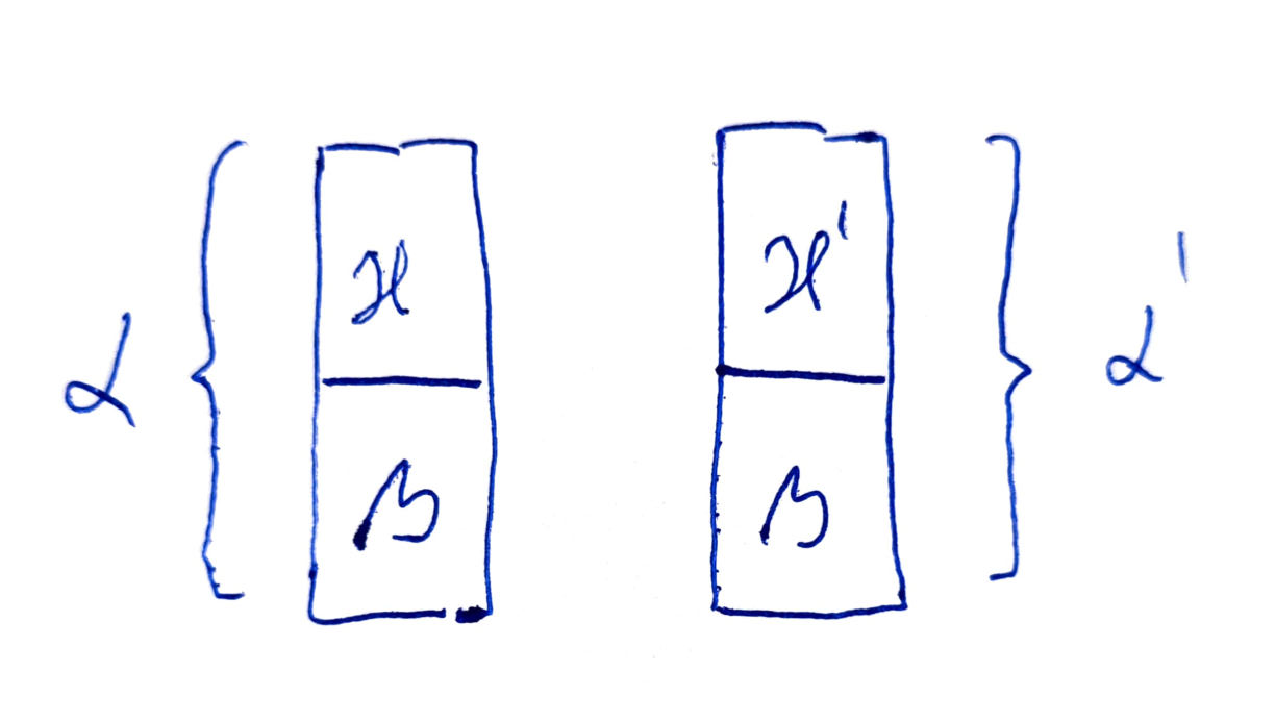
\includegraphics[width=0.35\linewidth]{rza_prechod_zasobnik.pdf}
    \caption{Stav zásobníku během přechodu RNZA. Platí $\alpha, \alpha', \beta, \gamma, \gamma' \in \Gamma^*$.}
\end{figure}

\subsection{Deterministický zásobníkový automat}

Deterministický zásobníkový automat (DZA) disponuje menší vyjadřovací sílou než NZA (resp. RNZA). Jazyky přijímané DZA označujeme jako deterministické bezkontextové jazyky ($\mathcal{L}_{DCF}$). Formálně: $\mathcal{L}_{DCF} \subset \mathcal{L}_2$ a tedy $\exists L \in \mathcal{L}_2 : L \not\in \mathcal{L}_{DCF}$.

\paragraph*{Definice} Zdroj nedeterminismu v NZA je volba znaku $a \in ( \Sigma \cup \{ \epsilon \} )$ při přechodu do další konfigurace. DZA se od NZA liší tvarem přechodové funkce, formálně:

$$ \forall q \in Q ~ \forall a \in \Sigma ~ \forall Z \in \Gamma ~:~ $$

$$ ~:~ ( ~ |\delta(q, a, Z)| \leq 1 ~\land~ | \delta(q, \epsilon, Z)| = 0 ) ~ \lor $$

$$ \lor ~ ( ~ |\delta(q, a, Z)| = 0 ~\land~ | \delta(q, \epsilon, Z)| \leq 1 ) $$

\paragraph*{Příklad} Příklad jazyka, který patří do $\mathcal{L}_{DCF}$, ale nepatří do $\mathcal{L}_{3}$.

$$L = a^n b^n ~;~ n \geq 0$$

\begin{figure}[H]
    \centering
    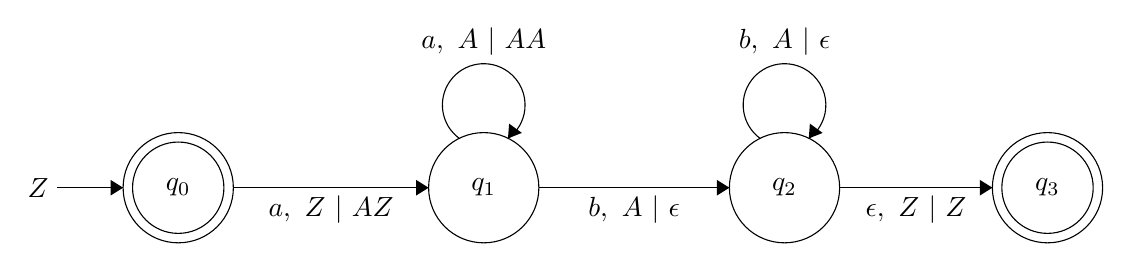
\begin{tikzpicture}[scale=0.2]
        \tikzstyle{every node}+=[inner sep=0pt]
        \draw [black] (14.4,-24.6) circle (3.5);
        \draw (14.4,-24.6) node {$q_0$};
        \draw [black] (14.4,-24.6) circle (2.9);
        \draw [black] (33.8,-24.6) circle (3.5);
        \draw (33.8,-24.6) node {$q_1$};
        \draw [black] (52.9,-24.6) circle (3.5);
        \draw (52.9,-24.6) node {$q_2$};
        \draw [black] (69.6,-24.6) circle (3.5);
        \draw (69.6,-24.6) node {$q_3$};
        \draw [black] (69.6,-24.6) circle (2.9);
        \draw [black] (17.9,-24.6) -- (30.3,-24.6);
        \fill [black] (30.3,-24.6) -- (29.5,-24.1) -- (29.5,-25.1);
        \draw (24.1,-25.1) node [below] {$a,\mbox{ }Z\mbox{ }|\mbox{ }AZ$};
        \draw [black] (37.3,-24.6) -- (49.4,-24.6);
        \fill [black] (49.4,-24.6) -- (48.6,-24.1) -- (48.6,-25.1);
        \draw (43.35,-25.1) node [below] {$b,\mbox{ }A\mbox{ }|\mbox{ }\epsilon$};
        \draw [black] (6.7,-24.6) -- (10.9,-24.6);
        \draw (6.2,-24.6) node [left] {$Z$};
        \fill [black] (10.9,-24.6) -- (10.1,-24.1) -- (10.1,-25.1);
        \draw [black] (32.257,-21.474) arc (234:-54:2.625);
        \draw (33.8,-16.23) node [above] {$a,\mbox{ }A\mbox{ }|\mbox{ }AA$};
        \fill [black] (35.34,-21.47) -- (36.22,-21.12) -- (35.41,-20.53);
        \draw [black] (51.357,-21.474) arc (234:-54:2.625);
        \draw (52.9,-16.23) node [above] {$b,\mbox{ }A\mbox{ }|\mbox{ }\epsilon$};
        \fill [black] (54.44,-21.47) -- (55.32,-21.12) -- (54.51,-20.53);
        \draw [black] (56.4,-24.6) -- (66.1,-24.6);
        \fill [black] (66.1,-24.6) -- (65.3,-24.1) -- (65.3,-25.1);
        \draw (61.25,-25.1) node [below] {$\epsilon,\mbox{ }Z\mbox{ }|\mbox{ }Z$};
    \end{tikzpicture}
    \caption{Příklad deterministického zásobníkového automatu.}
\end{figure}

\subsection{Deterministický rozšířený zásobníkový automat}

RNZA obsahuje více zdrojů nedeterminismu než NZA. Kromě možnosti volby $a \in ( \Sigma \cup \{ \epsilon \} )$ je to také volba $ \gamma \in \Gamma^* $. Tedy kolik znaků ze zásobníku bude zkonzumováno. \todo{todo}
